	%%%%%%%%%%%%%%%%%%%%%%%%%%%%%%%%%%%%%%%%%
% Cleese Assignment (For Students)
% LaTeX Template
% Version 2.0 (27/5/2018)
%
% This template originates from:
% http://www.LaTeXTemplates.com
%
% Author:
% Vel (vel@LaTeXTemplates.com)
%
% License:
% CC BY-NC-SA 3.0 (http://creativecommons.org/licenses/by-nc-sa/3.0/)
% 
%%%%%%%%%%%%%%%%%%%%%%%%%%%%%%%%%%%%%%%%%

%----------------------------------------------------------------------------------------
%	PACKAGES AND OTHER DOCUMENT CONFIGURATIONS
%----------------------------------------------------------------------------------------

\documentclass[11pt]{article}

%%%%%%%%%%%%%%%%%%%%%%%%%%%%%%%%%%%%%%%%%
% Cleese Assignment
% Structure Specification File
% Version 1.0 (27/5/2018)
%
% This template originates from:
% http://www.LaTeXTemplates.com
%
% Author:
% Vel (vel@LaTeXTemplates.com)
%
% License:
% CC BY-NC-SA 3.0 (http://creativecommons.org/licenses/by-nc-sa/3.0/)
% 
%%%%%%%%%%%%%%%%%%%%%%%%%%%%%%%%%%%%%%%%%

%----------------------------------------------------------------------------------------
%	PACKAGES AND OTHER DOCUMENT CONFIGURATIONS
%----------------------------------------------------------------------------------------

\usepackage{lastpage} % Required to determine the last page number for the footer

\usepackage{graphicx} % Required to insert images

\setlength\parindent{0pt} % Removes all indentation from paragraphs

\usepackage[most]{tcolorbox} % Required for boxes that split across pages

\usepackage{booktabs} % Required for better horizontal rules in tables

\usepackage{listings} % Required for insertion of code

\usepackage{etoolbox} % Required for if statements

\usepackage{amsmath}

\usepackage{listings}% http://ctan.org/pkg/listings

\newcommand{\dollar}{\mbox{\textdollar}}

\usepackage{qtree}

\usepackage{dramatist}

\usepackage{hyperref}

\usepackage[dvipsnames]{xcolor}


\lstset{
tabsize = 4, %% set tab space width
showstringspaces = false, %% prevent space marking in strings, string is defined as the text that is generally printed directly to the console
numbers = left, %% display line numbers on the left
commentstyle = \color{green}, %% set comment color
keywordstyle = \color{blue}, %% set keyword color
stringstyle = \color{red}, %% set string color
rulecolor = \color{black}, %% set frame color to avoid being affected by text color
basicstyle = \small \ttfamily , %% set listing font and size
breaklines = true, %% enable line breaking
numberstyle = \tiny,
commentstyle = \color{ForestGreen}
}

%----------------------------------------------------------------------------------------
%	MARGINS
%----------------------------------------------------------------------------------------

\usepackage{geometry} % Required for adjusting page dimensions and margins

\geometry{
	paper=a4paper, % Change to letterpaper for US letter
	top=3cm, % Top margin
	bottom=3cm, % Bottom margin
	left=2.5cm, % Left margin
	right=2.5cm, % Right margin
	headheight=14pt, % Header height
	footskip=1.4cm, % Space from the bottom margin to the baseline of the footer
	headsep=1.2cm, % Space from the top margin to the baseline of the header
	%showframe, % Uncomment to show how the type block is set on the page
}

%----------------------------------------------------------------------------------------
%	FONT
%----------------------------------------------------------------------------------------

\usepackage[utf8]{inputenc} % Required for inputting international characters
\usepackage[T1]{fontenc} % Output font encoding for international characters

\usepackage[sfdefault,light]{roboto} % Use the Roboto font

%----------------------------------------------------------------------------------------
%	HEADERS AND FOOTERS
%----------------------------------------------------------------------------------------

\usepackage{fancyhdr} % Required for customising headers and footers

\pagestyle{fancy} % Enable custom headers and footers

\lhead{\small\assignmentClass:\ifdef{\assignmentClassInstructor}{\ (\assignmentClassInstructor):}{}\ \assignmentTitle} % Left header; output the instructor in brackets if one was set
\chead{} % Centre header
\rhead{\small\ifdef{\assignmentAuthorName}{\assignmentAuthorName}{\ifdef{\assignmentDueDate}{Due\ \assignmentDueDate}{}}} % Right header; output the author name if one was set, otherwise the due date if that was set

\lfoot{} % Left footer
\cfoot{\small Page\ \thepage\ of\ \pageref{LastPage}} % Centre footer
\rfoot{} % Right footer

\renewcommand\headrulewidth{0.5pt} % Thickness of the header rule

%----------------------------------------------------------------------------------------
%	MODIFY SECTION STYLES
%----------------------------------------------------------------------------------------

\usepackage{titlesec} % Required for modifying sections

%------------------------------------------------
% Section

\titleformat
{\section} % Section type being modified
[block] % Shape type, can be: hang, block, display, runin, leftmargin, rightmargin, drop, wrap, frame
{\Large\bfseries} % Format of the whole section
{\assignmentQuestionName~\thesection} % Format of the section label
{6pt} % Space between the title and label
{} % Code before the label

\titlespacing{\section}{0pt}{0.5\baselineskip}{0.5\baselineskip} % Spacing around section titles, the order is: left, before and after

%------------------------------------------------
% Subsection

\titleformat
{\subsection} % Section type being modified
[block] % Shape type, can be: hang, block, display, runin, leftmargin, rightmargin, drop, wrap, frame
{\itshape} % Format of the whole section
{(\alph{subsection})} % Format of the section label
{4pt} % Space between the title and label
{} % Code before the label

\titlespacing{\subsection}{0pt}{0.5\baselineskip}{0.5\baselineskip} % Spacing around section titles, the order is: left, before and after

\renewcommand\thesubsection{(\alph{subsection})}

%----------------------------------------------------------------------------------------
%	CUSTOM QUESTION COMMANDS/ENVIRONMENTS
%----------------------------------------------------------------------------------------

% Environment to be used for each question in the assignment
\newenvironment{question}{
	\vspace{0.5\baselineskip} % Whitespace before the question
	\section{} % Blank section title (e.g. just Question 2)
	\lfoot{\small\itshape\assignmentQuestionName~\thesection~continued on next page\ldots} % Set the left footer to state the question continues on the next page, this is reset to nothing if it doesn't (below)
}{
	\lfoot{} % Reset the left footer to nothing if the current question does not continue on the next page
}

%------------------------------------------------

% Environment for subquestions, takes 1 argument - the name of the section
\newenvironment{subquestion}[1]{
	\subsection{#1}
}{
}

%------------------------------------------------

% Command to print a question sentence
\newcommand{\questiontext}[1]{
	\textbf{#1}
	\vspace{0.5\baselineskip} % Whitespace afterwards
}

%------------------------------------------------

% Command to print a box that breaks across pages with the question answer
\newcommand{\answer}[1]{
	\begin{tcolorbox}[breakable, enhanced, parbox=false]
		#1
	\end{tcolorbox}
}

%------------------------------------------------

% Command to print a box that breaks across pages with the space for a student to answer
\newcommand{\answerbox}[1]{
	\begin{tcolorbox}[breakable, enhanced]
		\vphantom{L}\vspace{\numexpr #1-1\relax\baselineskip} % \vphantom{L} to provide a typesetting strut with a height for the line, \numexpr to subtract user input by 1 to make it 0-based as this command is
	\end{tcolorbox}
}

%------------------------------------------------

% Command to print an assignment section title to split an assignment into major parts
\newcommand{\assignmentSection}[1]{
	{
		\centering % Centre the section title
		\vspace{2\baselineskip} % Whitespace before the entire section title
		
		\rule{0.8\textwidth}{0.5pt} % Horizontal rule
		
		\vspace{0.75\baselineskip} % Whitespace before the section title
		{\LARGE \MakeUppercase{#1}} % Section title, forced to be uppercase
		
		\rule{0.8\textwidth}{0.5pt} % Horizontal rule
		
		\vspace{\baselineskip} % Whitespace after the entire section title
	}
}

%----------------------------------------------------------------------------------------
%	TITLE PAGE
%----------------------------------------------------------------------------------------

\author{\textbf{\assignmentAuthorName}} % Set the default title page author field
\date{} % Don't use the default title page date field

\title{
	\thispagestyle{empty} % Suppress headers and footers
	\vspace{0.2\textheight} % Whitespace before the title
	\textbf{\assignmentClass:\ \assignmentTitle}\\[-4pt]
	\ifdef{\assignmentDueDate}{{\small Due\ on\ \assignmentDueDate}\\}{} % If a due date is supplied, output it
	\ifdef{\assignmentClassInstructor}{{\large \textit{\assignmentClassInstructor}}}{} % If an instructor is supplied, output it
	\vspace{0.32\textheight} % Whitespace before the author name
} % Include the file specifying the document structure and custom commands

%----------------------------------------------------------------------------------------
%	ASSIGNMENT INFORMATION
%----------------------------------------------------------------------------------------

% Required
\newcommand{\assignmentQuestionName}{Question} % The word to be used as a prefix to question numbers; example alternatives: Problem, Exercise
\newcommand{\assignmentClass}{Advanced Programming} % Course/class
\newcommand{\assignmentTitle}{JVM \& Tools} % Assignment title or name
\newcommand{\assignmentAuthorName}{Dario Bekic} % Student name


%----------------------------------------------------------------------------------------

\begin{document}

%----------------------------------------------------------------------------------------
%	TITLE PAGE
%----------------------------------------------------------------------------------------

\maketitle % Print the title page

\thispagestyle{empty} % Suppress headers and footers on the title page

\newpage

%----------------------------------------------------------------------------------------
%	QUESTION 1
%----------------------------------------------------------------------------------------

\begin{question}

\questiontext{Write a simple Java program JustCreate that in a very long loop creates at each iteration
one object, discarding immediately any reference to it.\\ Every 1000 iterations the program
must print the number of objects created since the beginning and must pause for 50
milliseconds (use e.g. Thread.sleep()).\\
Inspect the program execution with VisualVM, and try to tune the parameters so that the
heap occupancy profile has the shape of a shark's teeth}

\answer{To resemble a Shark's teeth we need an increasing phase, which corresponds to the allocation phase, and then a decreasing one. \\
To actually see the shark's teeth we need to decrease the difference between the heap allocated size for the jvm and the heap used by our $\textbf{java.lang.Object}$s.\\
To simplify we chose the serial garbage collector, which has an easier-to-predict behaviour w.r.t the newer and parallel counterparts.
With repeated tests, the application consumes $\approx$ 5Mb at the start of the application and at each sweep made by the GC, thus a 2Mb for Eden's space seemed appropriate.\\
}

\begin{lstlisting}[language=bash, caption={How to launch JustCreate},captionpos=b]
~$ java -XX:+UseSerialGC -Xmx8m JustCreate 
\end{lstlisting}              

\begin{figure}[h]
\centering
    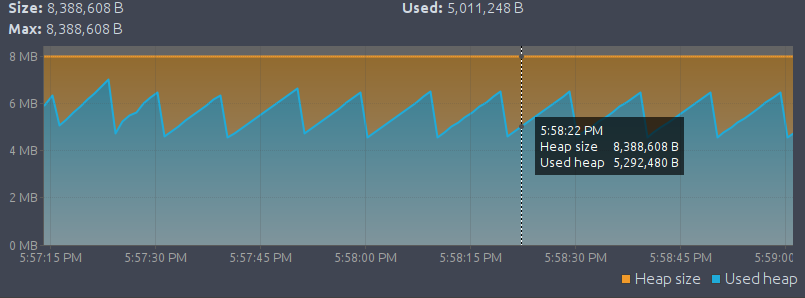
\includegraphics[width=1\textwidth]{images/Shark.png}
    \caption{Sharks teeth}
\end{figure}

\end{question}

\newpage

\begin{question}
    \questiontext{As we have seen recently, the JVM has two instructions that can be used to compile
a switch statement: \underline{tableswitch} and \underline{lookupswitch}. Taking inspiration from the
examples seen at lesson, try to determine when your Java compiler
uses \underline{tableswitch} and when it uses \underline{lookupswitch}.
Does this depend only on the distance between the smallest and the largest constants in
the case clauses? Are other criteria considered as well?
Use javap -c -v ClassName.class or godbolt.org to disassemble the compiled
bytecode.}



I found \href{https://github.com/openjdk/jdk/blob/082125d61e4b7e0fd53528c0271ca8be621f242b/src/jdk.compiler/share/classes/com/sun/tools/javac/jvm/Gen.java#L1350}{here} the source code which chooses how to pick which instruction to emit.

\begin{lstlisting}[language = Java , frame = trBL , firstnumber = last , escapeinside={(*@}{@*)}]
// Determine whether to issue a tableswitch or a lookupswitch 
// instruction.
        long table_space_cost = 4 + ((long) hi - lo + 1); // words
        long table_time_cost = 3; // comparisons
        long lookup_space_cost = 3 + 2 * (long) nlabels;
        long lookup_time_cost = nlabels;
        int opcode =
            nlabels > 0 &&
            table_space_cost + 3 * table_time_cost <=
            lookup_space_cost + 3 * lookup_time_cost
            ?
            tableswitch : lookupswitch;

\end{lstlisting}

It seems the difference between highest ($hi$) and lowest ($lo$) is only the space factor. The costants $3$ and $4$ are probably due to the space needed for emitting the two $\verb|switch|$ instructions. 
The space cost for the continuos jump table is correctly calculated as $hi-lo + 1$ considering the default clause and all other labels.\\
Lookup time cost is linear even though the JVM sorts the labels which could enable a binary search, however, it seems that the benefit for such implementation is not considered.
\end{question}

\begin{question}

\questiontext{Run the program WrongQueue and inspect its behaviour using VisualVM. Can you
explain the continuous growth of the heap? Find the code causing the bug and fix it.
Clearly, there are several ways to fix the bug: for this exercise, try to find one with minimal
“edit distance” from the source, i.e. the one obtained with the minimum amount of
character insertions or deletions.}

\verb|current| and \verb|head| represent semantically the same thing, but in the code of procedure \verb|dequeue| only \verb|current| is updated. Since \verb|head| keeps reference to the object pointed before by \verb|current| it cannot be garbage collected. I believe the minimum edit distance to make the program correct, in the sense that WrongQueue behaves like a FIFO Queue, is adding \verb|= head| in the second instruction of the \verb|dequeue| procedure.

\begin{lstlisting}[language = Java , frame = trBL , firstnumber = last , escapeinside={(*@}{@*)}]
public String dequeue(){
        String result = null;
        
        if(current != null){
            result = current.data;
            current = head = current.next;
        }

        return result;
	    
    }
\end{lstlisting}

\end{question}

\newpage

\begin{question}


    \questiontext{In the last lesson, the lecturer claimed that when compiling a switch based on a String
value, the Java compiler uses a hashing function for strings. Verify that this is true. Also,
try to understand the bytecode produced by the compiler: if the hash value coincides with
the hash of a string of a case clause, apparently an additional comparison between the two
strings is performed. Why is this necessary?
Using javap or godbolt.org, disassemble the compiled code to see if the lecturer is
right. Also, search in the Java or JVM Specification the precise place where this
compilation scheme is prescribed.
Goal: Reading disassembled bytecode; checking the Java/JVM specification.}

Indeed this happens, as shown in the \verb|visitStringSwitch| method \href{https://github.com/openjdk/jdk/blob/309b929147e7dddfa27879ff31b1eaad271def85/src/jdk.compiler/share/classes/com/sun/tools/javac/comp/Lower.java#L3940}{here} and \href{https://hg.openjdk.org/jdk7u/jdk7u/langtools/file/41b81b3e37cd/src/share/classes/com/sun/tools/javac/comp/Lower.java#l3397}{here}.\\
The additional check is necessary because of potential problems regarding hashing, e.g. collisions, so an additional check is made using the \verb|String.equals| method.


\end{question}

\begin{question}
\questiontext{Exploring threads. Explore the threads of a running application using VisualVM. Write
a simple multi-threaded program which spawns a new thread every few second. Monitor
the threads, their state and the code they are executing using the thread monitor of
VisualVM and the Thread Dump facility. Look for information about the threads dedicated
to JIT compilation and to GC}

To JIT compilation are dedicated two threads, taken from a random thread dump:
\begin{lstlisting}
"C1 CompilerThread0" #17 [27735] daemon prio=9 os_prio=0 cpu=1276,54ms elapsed=79,64s tid=0x00007dbbdc15d550 nid=27735 waiting on condition  [0x0000000000000000]
   java.lang.Thread.State: RUNNABLE
   No compile task

   Locked ownable synchronizers:
        - None

\end{lstlisting}

and 

\begin{lstlisting}
"C2 CompilerThread0" #14 [27734] daemon prio=9 os_prio=0 cpu=3451,28ms elapsed=79,64s tid=0x00007dbbdc15be40 nid=27734 waiting on condition  [0x0000000000000000]
   java.lang.Thread.State: RUNNABLE
   No compile task

   Locked ownable synchronizers:
        - None

\end{lstlisting}

For Garbage Collection we have the \verb|Finalizer| thread which performs method \verb|Finalize| on unreachable objects.

It is possible to get the logs of the JIT threads adding the following parameters to the $\verb|java|$ command:

\begin{lstlisting}[language=bash, caption={Parameters for logging JIT Threads activities}]
XX:+UnlockDiagnosticVMOptions -XX+LogCompilation
\end{lstlisting}
\newpage
Each thread in my application calls the following method:
\begin{lstlisting}[language = Java , frame = trBL , firstnumber = last , escapeinside={(*@}{@*)}]
public int stupid() {
    int i=0;
    while (i<10000) {
        i = i + 1;
    }
    System.out.println("done");
}
\end{lstlisting}

The first reference we find about the method $\verb|stupid|$ is the following:
\begin{lstlisting}
<task_queued compile_id='6' compile_kind='osr' method='lol stupid ()V' bytes='25' count='7' backedge_count='60416' iicount='7' osr_bci='2' level='3' stamp='2,646' comment='tiered' hot_count='60416'/>
\end{lstlisting}

We observe that it is queued an OSR(i.e. On Stack Replecement) which is a request to the immediate replacement of interpretation with a compiled version of the method, this is done because the $\verb|while|$ is detected having lot of iterations($\verb|backedge_count='60416'|$).

\end{question}

\end{document}